\section{Distance measures for quantum information}
\textit{What does it mean to say that two items of information are similar? What does it mean to say that information is preserved by some process?} These questions are central to a theory of quantum information processing, and the purpose of this chapter is the development of distance measures giving quantitative answers to these questions. Motivated by our two questions we will be concerned with two broad classes of distance measures, \textit{static measures} and \textit{dynamic measures}. Static measures quantify how close two quantum states are, while dynamic measures quantify how well information has been preserved during a dynamic process.

\subsection{Distance measures for classical information}
One way of quantifying the distance between two strings of bits is the \textit{Hamming distance}, defined to be the number of places at which two bit strings are not equal. For example, the bit strings $00010$ and $10011$ differ in the first and last place, so the Hamming distance between them is two. Unfortunately, the Hamming distance between two objects is simply a matter of labeling, and \textit{a priori} there aren't any labels in the Hilbert space arena of quantum mechanics!
\vspace{1em}

The first measure is the \textit{trace distance,} defined by the equation:
$$D(p_x, q_x) \equiv \frac{1}{2}\sum_x{|p_x-q_x|}$$
This quantity is sometimes known as the $L_1$ distance or \textit{Kolmogorov distance}. The trace distance turns out to be a metric on probability distributions, so the use of the term 'distance' is justified.
\vspace{1em}

A second measure of distance between probability distributions, the \textit{fidelity} of the probability distributions $\{p_x\}$ and $\{q_x\}$, is defined by
$$F(p_x, q_x) \equiv \sum_x{\sqrt{p_x q_x}}$$

The fidelity is a very different way of measuring distance between probability distributions
than is the trace distance. The fidelity is just the inner product between vectors with components $\sqrt{p_x}$ and $\sqrt{q_x}$, which lie on a unit sphere.
\begin{figure}[h]
    \centering
    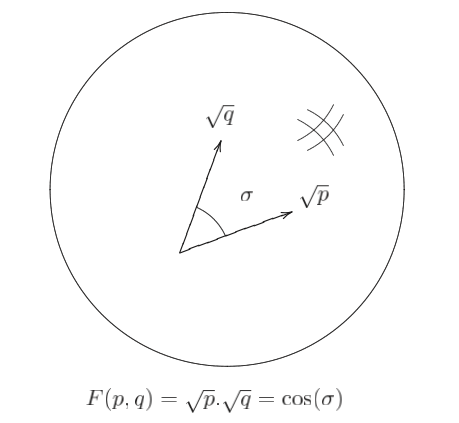
\includegraphics[width=0.4\textwidth]{fidelity.png}
    \caption{Geometric interpretation of the fidelity as the inner product between vectors $\sqrt{p_x}$ and $\sqrt{q_x}$ lying on a unit sphere.}
\end{figure}

\newpage
\subsection{How close are two quantum states?}

\subsubsection{Trace}
Analogous to the classical case, we begin by defining the \textit{trace distance} between quantum states $\rho$ and $\sigma$,
$$D(\rho, \sigma) \equiv \frac{1}{2}\tr|\rho - \sigma|$$
where as per usual we define $|A| \equiv \sqrt{A^\dag A}$ to be the positive square root of $A^\dag A$. Notice that the quantum trace distance generalizes the classical trace distance in the sense that if $\rho$ and $\sigma$ commute then the (quantum) trace distance between $\rho$ and $\sigma$ is equal to the classical trace distance between the eigenvalues of $\rho$ and $\sigma$. More explicitly, if $\rho$ and $\sigma$ commute they are diagonal in the same basis,
$$\rho = \sum_i{r_i\ket{i}\bra{i}};\ \sigma = \sum_i{s_i\ket{i}\bra{i}},$$
for some orthonormal basis $\ket{i}$. Thus
\begin{equation*}
\begin{split}
    D(\rho, \sigma) & = \frac{1}{2}\tr|\sum_i{(r_i - s_i)\ket{i}\bra{i}}|\\
    & = D(r_i, s_i)
\end{split}
\end{equation*}

\begin{theorem}
    Let $\{E_m\}$ be a POVM, with $p_m \equiv \tr(\rho E_m)$ and $q_m \equiv \tr(\sigma E_m)$ as the probabilities of obtaining a measurement outcome labeled by $m$. Then
    $$D(\rho, \sigma) = \max_{\{E_m\}}D(p_m, q_m)$$
    where the maximization is over all POVMs $\{E_m\}$.
\end{theorem}
\begin{proof}
    Note that
    $$D(p_m, q_m) = \frac{1}{2} \sum_m|\tr(E_m(\rho − \sigma))|$$
    Using the spectral decomposition we may write $\rho − \sigma = Q − S$, where $Q$ and $S$ are positive operators with orthogonal support. Thus $|\rho − \sigma| = Q + S$, and
    \begin{equation*}
    \begin{split}
        |tr(E_m(\rho − \sigma))| & = |\tr(E_m(Q - S))|\\
        & \leq |\tr(E_m(Q + S))|\\
        & \leq |\tr(E_m|\rho - \sigma|)|
    \end{split}
    \end{equation*}
    Thus
    \begin{equation*}
    \begin{split}
        D(p_m, q_m) & \leq \frac{1}{2} \sum_m{\tr(E_m|\rho − \sigma|)}\\
        & = \frac{1}{2}\tr|\rho - \sigma|\\
        & = D(\rho, \sigma)
    \end{split}
    \end{equation*}
    where we have applied the completeness relation for POVM elements, $\sum_m{E_m} = I$.\\
    Conversely, by choosing a measurement whose POVM elements include projectors onto the support of $Q$ and $S$, we see that there exist measurements which give rise to probability distributions such that $D(p_m, q_m) = D(\rho, \sigma)$.
\end{proof}

\newpage
\subsubsection{Fidelity}

A second measure of distance between quantum states is the \textit{fidelity}. The fidelity of states $\rho$ and $\sigma$ is defined to be
$$F(\rho,\sigma) ≡ tr\sqrt{\rho^{1/2}\sigma\rho^{1/2}}$$
\begin{theorem}
    \textbf{(Uhlmann’s theorem)} Suppose $\rho$ and $\sigma$ are states of a quantum system $Q$. Introduce a second quantum system $R$ which is a copy of $Q$. Then
    $$F(\rho, \sigma)= max_{\ket{\psi}, \ket{\phi}} |\braket{\psi}{\phi}|$$
    where the maximization is over all purifications $\ket{\psi}$ of $\rho$ and $\ket{\phi}$ of $\sigma$ into $RQ$.
\end{theorem}
\begin{theorem}
    \textbf{(Monotonicity of the fidelity)} Suppose $\mathcal{E}$ is a trace-preserving quantum operation. Let $\rho$ and $\sigma$ be density operators. Show that
    $$F(\mathcal{E}(\rho), \mathcal{E}(\sigma)) \geq F(\rho, \sigma)$$
\end{theorem}
\begin{proof}
    Let $\ket{\psi}$ and $\ket{\phi}$ be purifications of $\rho$ and $\sigma$ into a joint system $RQ$ such that $F(\rho, \sigma) = |\braket{\psi}{\phi}|$. Introduce a model environment $E$ for the quantum operation, $\mathcal{E}$, which starts in a pure state $\ket{0}$, and interacts with the quantum system $Q$ via a unitary interaction $U$. Note that $U\ket{\psi}\ket{0}$ is a purification of $\mathcal{E}\rho$, and $U\ket{\phi}\ket{0}$ is a purification of $\mathcal{E}\sigma$. By Uhlmann's theorem it follows that
    \begin{equation*}
    \begin{split}
        F(\mathcal{E}\rho, \mathcal{E}\sigma) & \geq |\bra{\psi}\bra{0}U^\dag U\ket{\phi}\ket{0}|\\
        & = |\braket{\psi}{\phi}|\\
        & = F(\rho, \sigma)
    \end{split}
    \end{equation*}
\end{proof}